
\chapter{Implementation}
\label{sec:implementation}
\noindent
In this chapter, we provide a detailed implementation of our proposed methodology. We start by giving insight into the introduced algorithms for generating the synthetic datasets to train and test our models. Then we present the software platform we incorporated to shape and design our architectures. Finally, we demonstrate our networks' architecture and settings in detail. 

%\noindent In this chapter, we provide a detailed implementation of our proposed methodology. We start with presenting the software platform we incorporated to shape and design our models. Then we demonstrate our network's architecture in detail. Finally, we attempt to give insight into the datasets we used to train and test our model. 



\section{The Datasets}
\label{dataha}

Here we delve into the data processing part of this work by introducing three different datasets we created or applied for our empirical experiments. To that end, we provide a detailed explanation for each step of synthetic data generation process along with approaches and methods used to improve each dataset.

%Here we delve into the data processing part of this work by introducing three different datasets we generated or chose for our empirical experiments. To that end, we provide a detailed explanation of the approaches and methods used to generate and improve each dataset.

\subsection{Even-odd Digits Dataset}
\label{subsubsec:digit}

Our Even-odd handwritten dataset contains images of size $100\times100$. Each image is filled with from 0 up to 15 randomly selected digits from MNIST hand-written digits dataset. The process of creating images follows the steps in below:
\begin{enumerate}
\item MNIST Digits are resized to $18\times18$ pixels.
\item Up to 15 digits are randomly put in images of size $100\times100$ pixels.
\item The images are created with controlled overlapping by ensuring that two different numbers are 18 pixels away from each other, i.e. the distance between two digits centers is larger than 18 pixels.
\item Images are labeled with the number of even digits present in each image. 
\item The images are created uniformly, meaning that for example, the number of images containing 0 even digits is equal to the number of images containing 15 even digits.
\end{enumerate}
 This dataset has in total 1 million images: 800,000 images for training set and 200,000 as the test. Figure~\ref{fig:l2cmnist} illustrates some examples of even-odd digits dataset with different number of even digits in images.

\begin{figure}[H]
	\centering
	{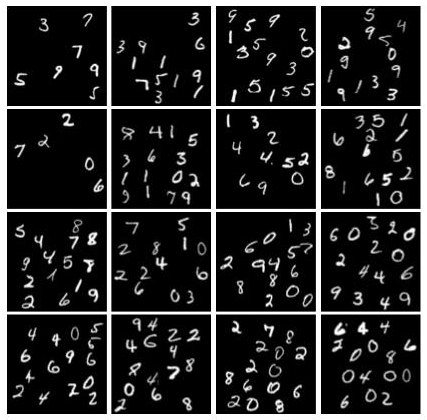
\includegraphics[width=0.5\textwidth]{images/l2cimages}}
		\caption{An example of even-odd digits images. Form left to right, images contain 0 to 15 even digits.}
	\label{fig:l2cmnist}
\end{figure}

%Digits are resized to $18\times18$ pixels and randomly put in the image. The images are created with controlled overlapping by ensuring that two different numbers are 18 pixels away from each other, i.e. the distance between two digits centers is larger than 18 pixels. For the training process, images are labeled with the number of even digits present in each image. Figure~\ref{fig:l2cmnist} illustrates some examples of even-odd digits dataset with different number of even digits in images.

%Our Even-odd handwritten dataset contains images of size $100\times100$. Each image is filled with from 0 up to 15 randomly selected digits from MNIST hand-written digits dataset. Digits are resized to $18\times18$ pixels and randomly put in the image. The images are created with controlled overlapping by ensuring that two different numbers are 18 pixels away from each other, i.e. the distance between two digits centers is larger than 18 pixels. For the training process, images are labeled with the number of even digits present in each image. Figure~\ref{fig:l2cmnist} illustrates some examples of even-odd digits dataset with different number of even digits in images. 

%\begin{figure}[H]
%	\centering
%	{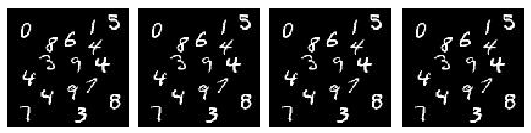
\includegraphics[width=0.9\textwidth]{images/l2cmnist}}
%		\caption{An example of even-odd digits images. Form left to right, images contain 0, 5, 10 and 15 even digits.}
%	\label{fig:l2cmnist}
%\end{figure}

%\indent This dataset has in total 1 million images: 800,000 images for training set and 200,000 as the test. Also, the dataset is uniformly generated, meaning that for instance, the number of images containing 0 even digits is \todo{`the numer' is always `is'} equal to the number of images containing 15 even digits.  

\subsection{Synthetic Pedestrians Dataset}
\label{subsec:synped}

Learning features using deep architectures requires a large amount of data. More importantly, for a fully supervised learning, this data should be annotated. Lack of data or its' high annotation cost prohibit the usage of deep learning methods for many problems including crowd counting. 

\indent However, in order to lower this cost, in our research, we decided to create a synthetic dataset of pedestrians in a walkway. To do that, we used UCSD unlabeled Anomaly detection dataset of pedestrians collected by \citeauthor{chan2008privacy} and used in \cite{chan2009analysis, mahadevan2010anomaly, li2014anomaly}. UCSD Anomaly detection dataset contains clips of groups of people walking towards and away from the camera, and consists of 34 training video samples and 36 testing video samples. Each video has 200 frames of each $238\times158$ pixels. Figure~\ref{fig:anomaly} depicts some images of UCSD Anomaly dataset.

\begin{figure}[H]
	\centering
	{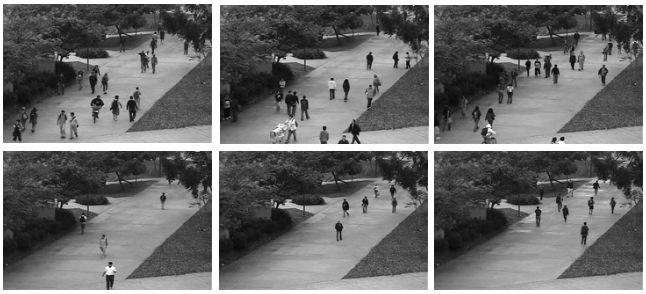
\includegraphics[width=0.7\textwidth]{images/anomaly}}
	\caption{Sample images of UCSD Anomaly detection dataset.}
	\label{fig:anomaly}
\end{figure}


\indent In our study, we used all 70 training and testing video samples to generate the synthetic pedestrians dataset. To thoroughly demonstrate the generation process of our dataset, we divide this section into data generation and data improvement.

  
\subsubsection{Data Generation}

In our dataset, we constrained each image by having up to 29 pedestrians in the walkway. The process of generating the data includes the following steps:
\begin{enumerate}

\item \textbf{Background extraction:} Firstly, we simply subtract the background from each video frame. We extract two types of backgrounds: the median of all the backgrounds in each video (in total, 70 different backgrounds), and the median of all median backgrounds. An example of extracted backgrounds is shown below.

\begin{figure}[H]
	\centering
	{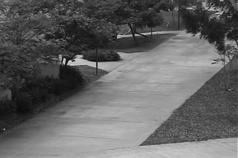
\includegraphics[width=0.4\textwidth]{images/background}}
	\caption{One background image extracted from UCSD dataset.}
	\label{fig:bgim}
\end{figure}


\item \textbf{Pedestrian extraction:} Subtracting each image from the mean background, we were able to label the connected regions (each individual in case of our images) of the subtraction using morphological labeling methods. Figure~\ref{fig:nobg} shows how images look like after background subtraction. 
\begin{figure}[H]
	\centering
	{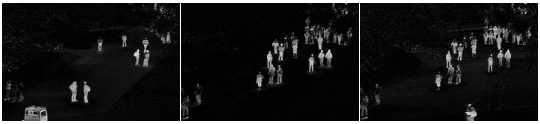
\includegraphics[width=0.9\textwidth]{images/nobg}}
	\caption{Images after background subtraction.}
	\label{fig:nobg}
\end{figure}
 
Then, properties of labeled regions are measured and bound-boxed (see \cite{van2014scikit} for more detailed explanation). Boxes of people are center-based annotated. These labeled boxes shape our initial list of pedestrians with masks of the same size of each box. Figure~\ref{backback} in below demonstrates a selection of extracted pedestrians and pedestrians' masks.

\begin{figure*}[h!]
    \centering
    \begin{subfigure}[t]{0.5\textwidth}
        \centering
        {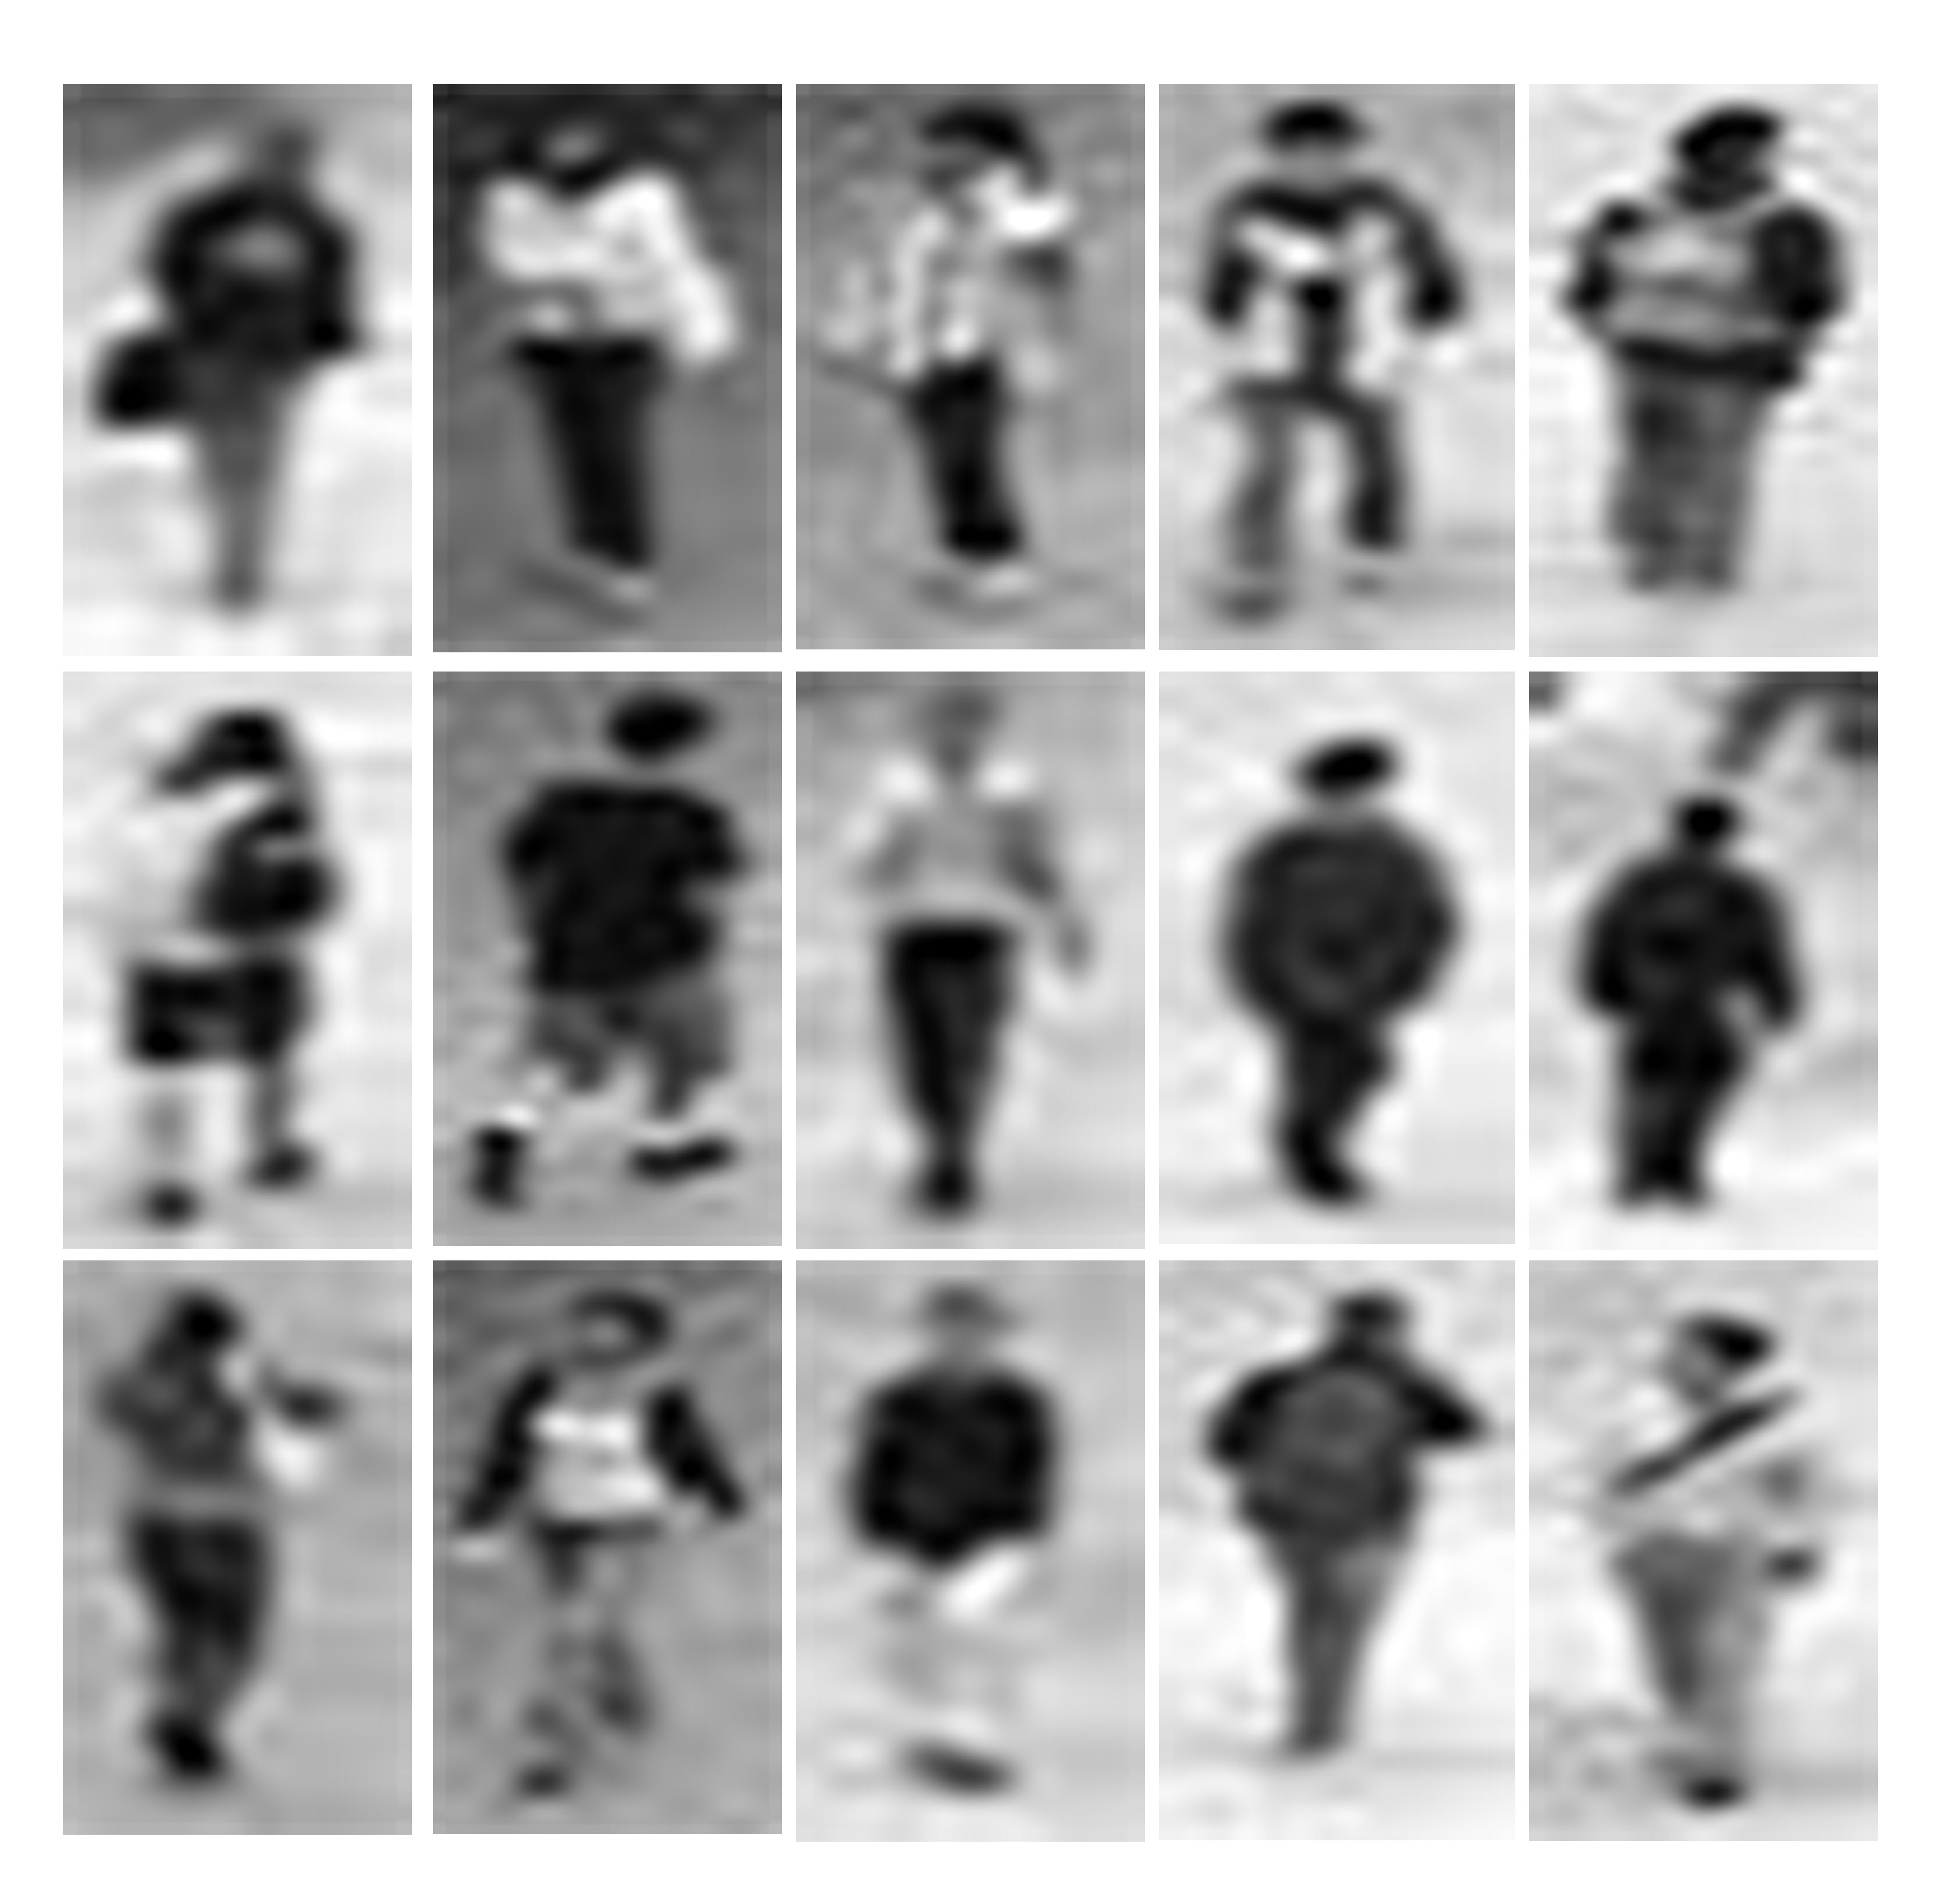
\includegraphics[width=0.5\textwidth]{images/peds}}
        \caption{Extracted pedestrians.}
    \end{subfigure}%
    ~ 
    \begin{subfigure}[t]{0.5\textwidth}
        \centering
        {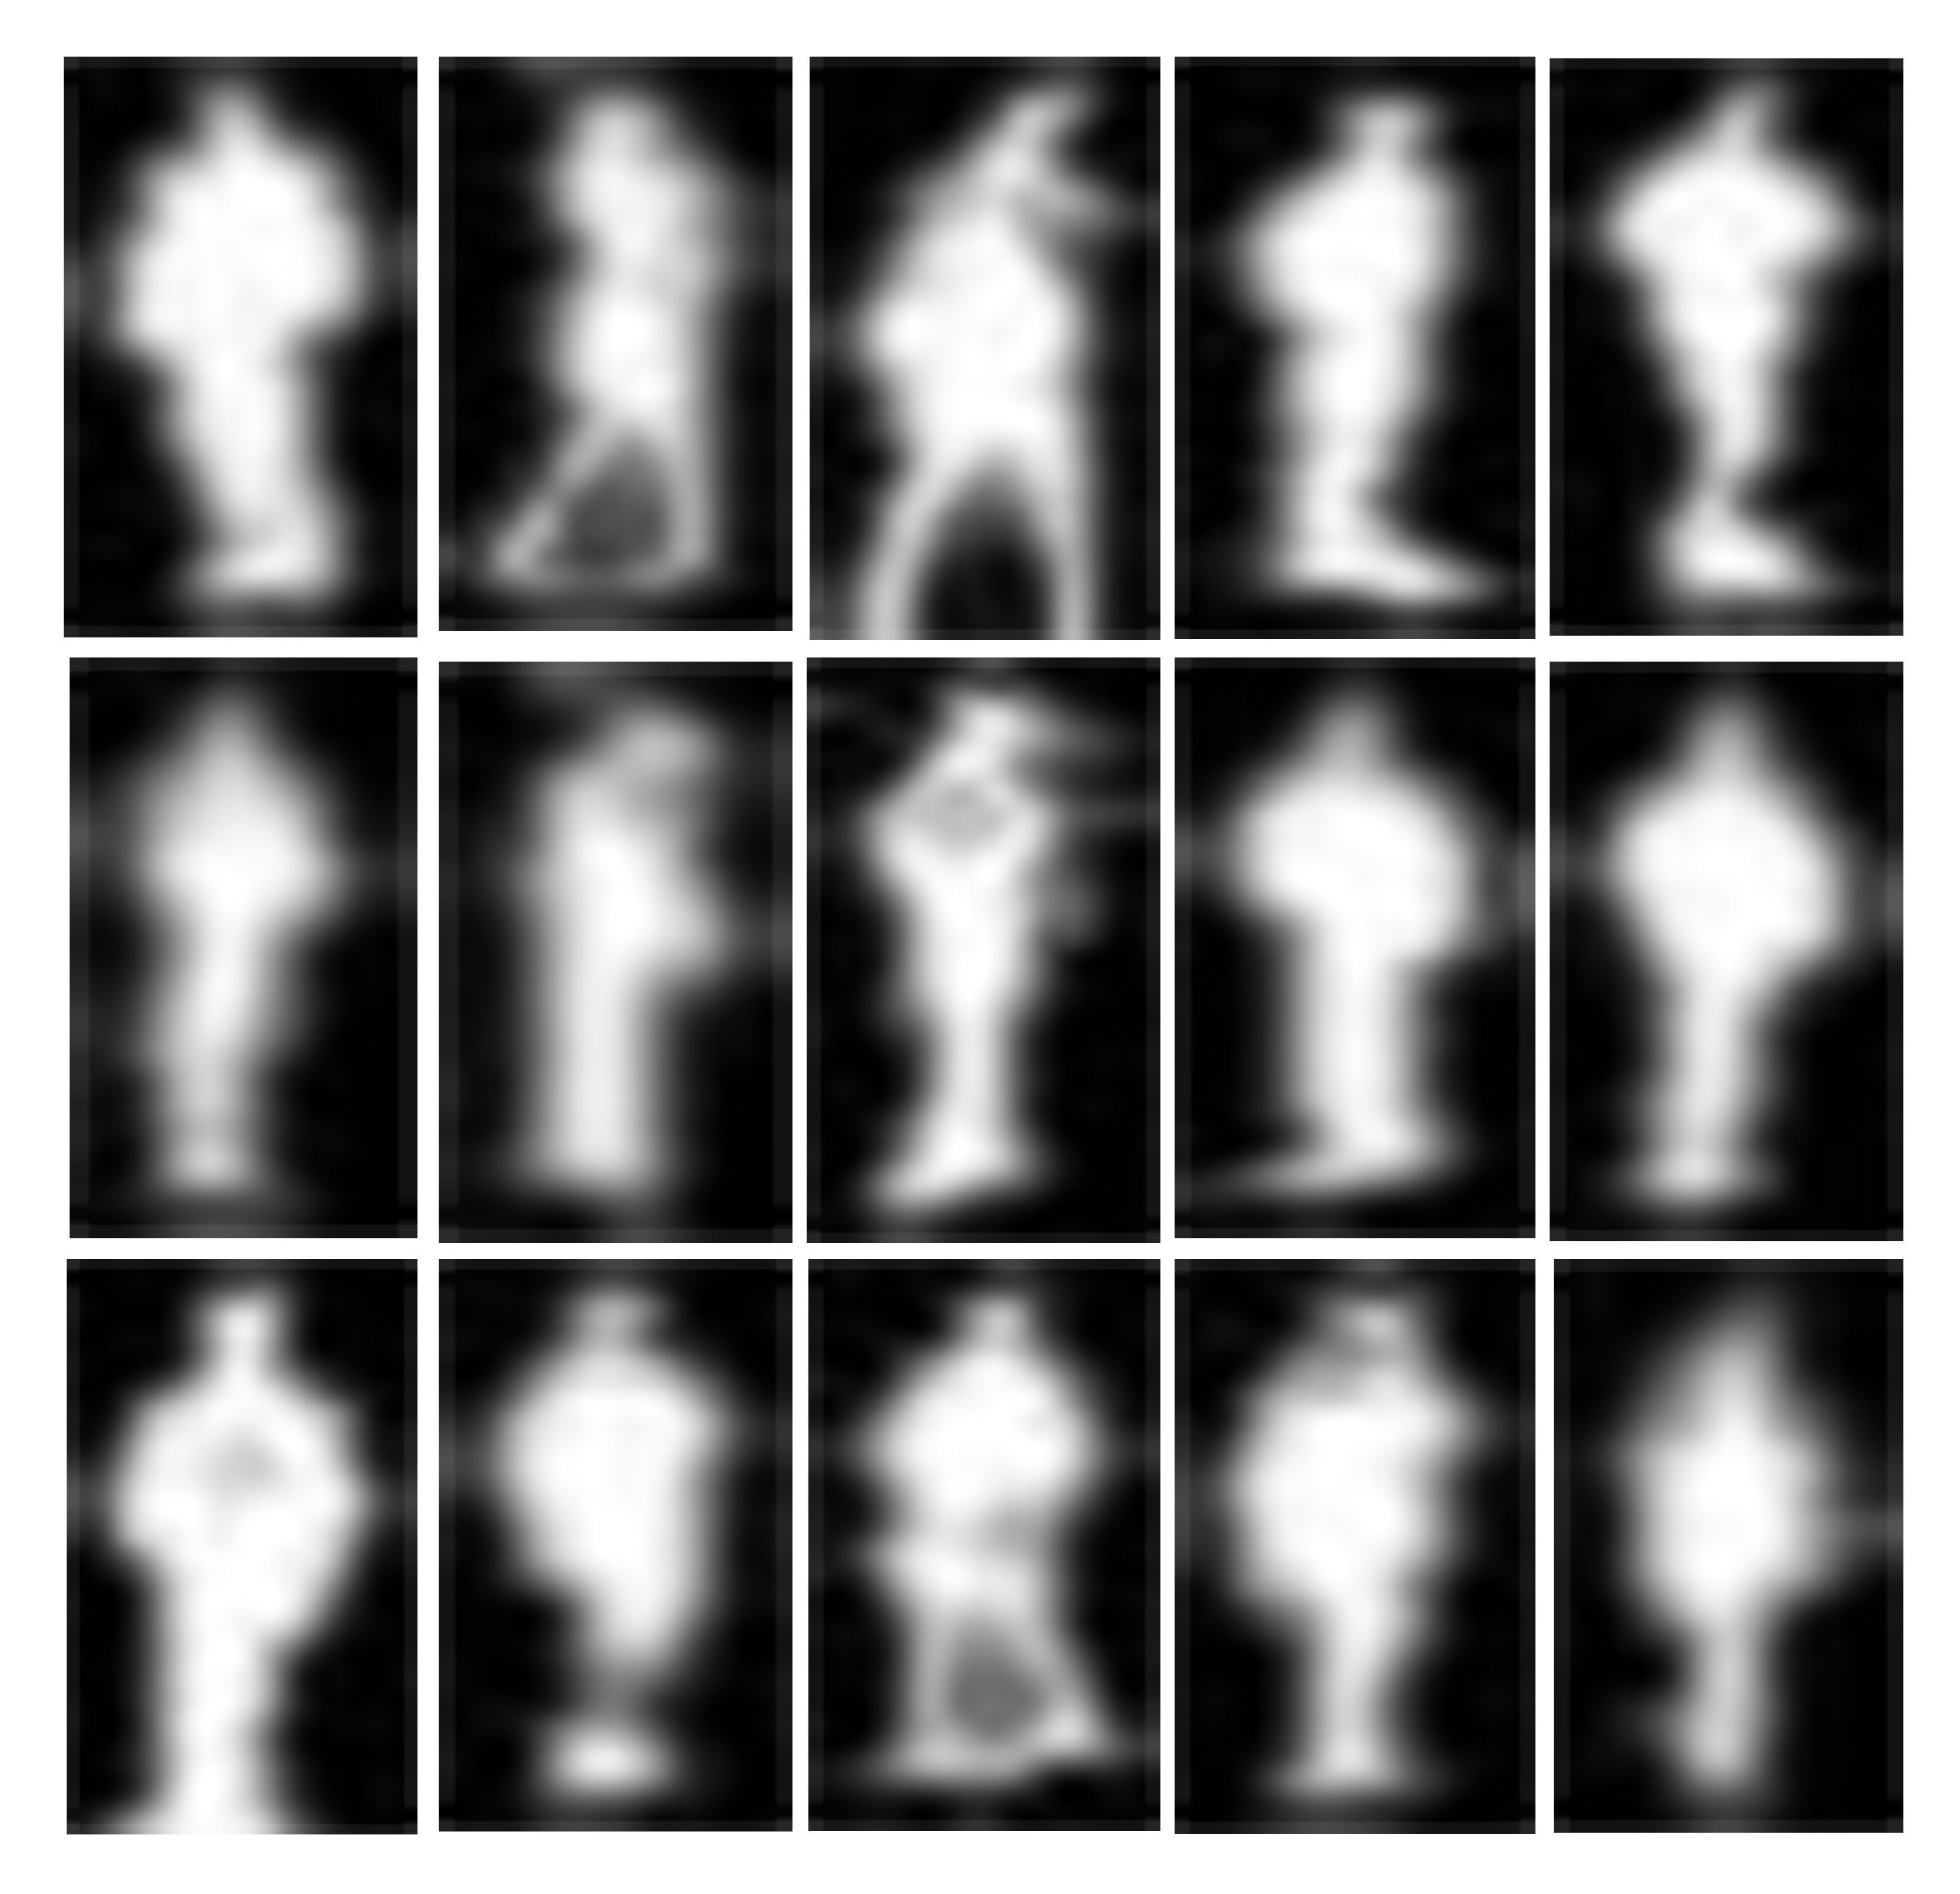
\includegraphics[width=0.5\textwidth]{images/masks}}
        \caption{created pedestrians' masks.}
    \end{subfigure}
    \caption{Pedestrians and their corresponding masks.}
    \label{backback}
\end{figure*}


\item \textbf{Background generation:} In this step, we tried to make the backgrounds of images as realistic as possible by:
\begin{enumerate}
\item making a sparse combination of median backgrounds.
\item changing the global illumination of the images randomly.
\item adding some random Gaussian noise to the backgrounds.
\end{enumerate}
 As you may notice, in the figure~\ref{backback}, the generated background happened to be brighter and noisier than the extracted one.
 
 
%1)~making a sparse combination of median backgrounds, 2)~changing the global illumination of the images randomly, and 3)~adding some \textit{Gaussian noise} to the backgrounds. As you may notice, in the figure~\ref{backback}, the generated background happened to be brighter and noisier than the extracted one. 

\begin{figure*}[h!]
    \centering
    \begin{subfigure}[t]{0.4\textwidth}
        \centering
        {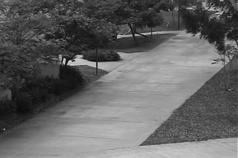
\includegraphics[width=0.8\textwidth]{images/background}}
        \caption{Raw extracted background image.}
    \end{subfigure}%
    ~ 
    \begin{subfigure}[t]{0.4\textwidth}
        \centering
        {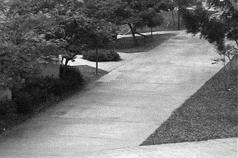
\includegraphics[width=0.8\textwidth]{images/background3}}
        \caption{Generated background after a sparse combination, global illumination change and some noise.}
    \end{subfigure}
    \caption{A synthetically generated background image}
    \label{backback}
\end{figure*}

 Having backgrounds generated and pedestrians extracted and labeled, backgrounds are selected randomly. Then, for training and comparison purposes, images are masked with a filter of \textit{Region Of Interest}~(ROI). The mask and ROI is shown in below (figure~\ref{fig:roi}).

\begin{figure*}[h!]
    \centering
    \begin{subfigure}[t]{0.4\textwidth}
        \centering
        {
\includegraphics[width=0.8\textwidth]{images/catwalk}}
        \caption{ROI mask.}
    \end{subfigure}%
    ~ 
    \begin{subfigure}[t]{0.4\textwidth}
        \centering
        {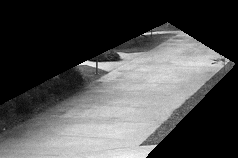
\includegraphics[width=0.8\textwidth]{images/roi}}
        \caption{ROI in the image.}
    \end{subfigure}
    \caption{Applying the mask of region of interest on the background image.}
    \label{fig:roi}
\end{figure*}

\item \textbf{Creating synthetic images:} Afterwards, pedestrians are added to the masked background in a way that the center of each person is placed inside white area of the mask. Finally images are normalized (between 0 and 255) and resized to $158\times158$ in order to be fed to convolution layers. A selection of created images are depicted in the figure underneath.

\begin{figure}[H]
	\centering
	{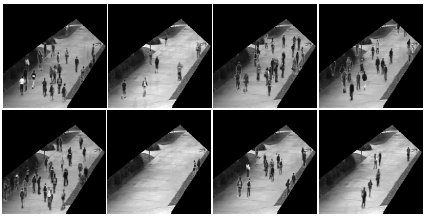
\includegraphics[width=0.8\textwidth]{images/myped}}
	\caption{created synthetic images for counting pedestrians problem.}
	\label{fig:myped}
\end{figure}

\end{enumerate}

\subsubsection{Data Improvement}
\label{dataimp}
Although we managed to successfully create synthetic images of people in the street, the generated images were still quite distinguishable from the real dataset. Thus, in order to make images as highly realistic as possible, we improved the dataset as explained underneath:
\begin{itemize}
\item \textbf{Non-pedestrian objects:} Amongst the extracted boxes of pedestrians, there were some non-pedestrian boxes with objects instead of pedestrians, and yet others with more than one person inside the box. Therefore, we manually removed these outliers. After this edition, we ended with 426 samples of people. A few examples of incorrectly collected or labeled objects are shown in below.

\begin{figure}[H]
	\centering
	{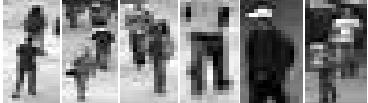
\includegraphics[width=0.6\textwidth]{images/nonped}}
	\caption{A selection of non-human or incorrectly labeled objects. As you may see, there are some images with "half a person" and some others with more than just one person in the image.}
	\label{fig:nonped}
\end{figure}
 
\item \textbf{Lack of pedestrians:} For the sake of generalization, we needed a decent variety of pedestrians in the images to train with. For this purpose, we created 2 versions of current pedestrians list, each darkened by the factor of 20\% from each other. 
\item \textbf{Halos around the pedestrians:} Due to lack of accuracy of the region measuring method, a fine layer of the background that pedestrians were extracted from, still remained around the pedestrians. In the created images, depending on where the person was placed, these thin layers appeared like a halo around the person. Figure~\ref{fig:haloim} illustrates some images with halos around the pedestrians. 
\begin{figure}[H]
	\centering
	{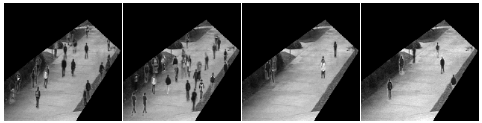
\includegraphics[width=0.8\textwidth]{images/halo}}
	\caption{A few synthetic images with halos around the pedestrians in the walkway.}
	\label{fig:haloim}
\end{figure}
 
To mitigate this issue, we tried two approaches:
\begin{enumerate}
\item \textbf{Morphological erosion:} Among morphological operations on image, we applied \textit{erosion} \cite{van2014scikit} to erode the pedestrians masks. In this way, the halos were ignored to some noticeable extent. 
\item \textbf{Poisson image editing:} Poisson image editing is a technique for seamlessly blending two images together fully automatically  \cite{perez2003poisson}. In addition to erosion, we tried Poisson image editing tool to remove the halos. However, due to our gray-scale and low-resolution images, this tool did not have a great impact on our images.      
\end{enumerate}
Afterwards, the images look similar to the ones shown in figure~\ref{fig:nohalo}.

\begin{figure}[H]
	\centering
	{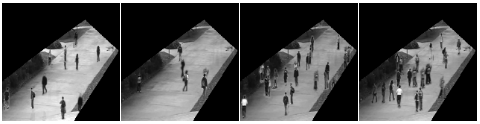
\includegraphics[width=0.8\textwidth]{images/nohalo}}
	\caption{Some examples of images with no or less halo around the people in the images.}
	\label{fig:nohalo}
\end{figure}
 
\item \textbf{Image Perspective:} Since pedestrians of different sizes were put randomly in the images, we considered people's tallness perspective in the images. As you may observe, in the following figure~\ref{fig:nopers}, image perspective has not been applied in the images and hence, there are some pedestrians closer to the camera but really small and also some pedestrians quite tall at the end of walkway.

\begin{figure}[H]
	\centering
	{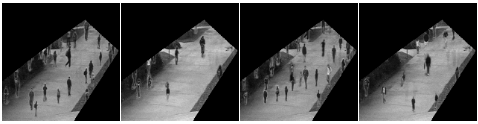
\includegraphics[width=0.8\textwidth]{images/nopers}}
	\caption{created images before considering image perspective.}
	\label{fig:nopers}
\end{figure}

Humans' height almost follows a Gaussian distribution \cite{subramanian2011height}. Therefore, with respect to \cite{subramanian2011height, garcia2007evolution}, we mapped individual's heights with the length of the walkway in the image, considering a Gaussian noise with mean $\mu = 0$ and $\sigma = 3.5$. The resulting images are demonstrated as follows.

\begin{figure}[H]
	\centering
	{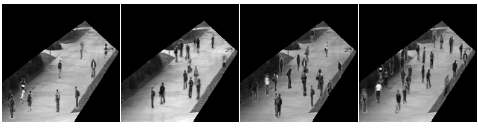
\includegraphics[width=0.8\textwidth]{images/pers}}
	\caption{Synthetic images considering image perspective based on the real distribution of people's height. As you may see, after applying perspective, the images look more realistic. }
	\label{fig:pers}
\end{figure}


\end{itemize}

\noindent Thusly, we created a set of 1 million images, each of size $158\times158$ pixels with up to 29 pedestrians. We assigned 800,000 images for training set and 200,000 instances as the test set. We believe the created synthetic dataset of pedestrians is realistic enough to be able to represent a real-world crowd counting scenario. However, the images can be improved in different aspects and by using diverse image editing and manipulation techniques. 

\subsection{UCSD Crowd counting Dataset}
\label{subsec:datareal2}
To verify and validate our model, we used UCSD crowd counting dataset created by \citeauthor*{chan2008privacy} and used in \cite{chan2008privacy,chan2009bayesian,chan2012counting}. The dataset contains video of pedestrians on UCSD walkways, taken from a stationary camera. There are currently two  viewpoints available among which we used \textit{vidf} videos. All videos are 8-bit gray-scale, each video file has 200 video frames, with dimensions $238\times158$. In our experiment, the first 20 videos which are labeled with the number of pedestrians, were incorporated. The center point of each pedestrian defines its' location in the image. A selection of UCSD crowd counting images is shown in figure~\ref{fig:ucsdorg}.

\begin{figure}[H]
	\centering
	{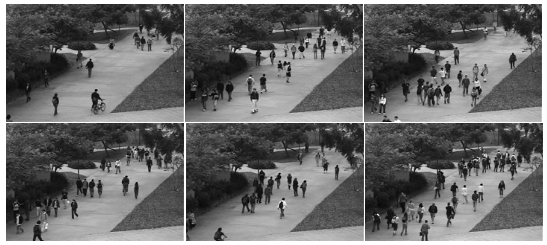
\includegraphics[width=0.8\textwidth]{images/normalucsd}}
	\caption{Normal UCSD crowd counting dataset images.}
	\label{fig:ucsdorg}
\end{figure}

\indent Among the labeled images, we selected the ones in which the number of pedestrians does not exceed 29. Then, images were resized to  $158\times158$ pixels and normalized between 0 and 255. Hence, in total we have a dataset of 3375 real images which are masked with the same filter we used for synthetic pedestrians dataset (shown in figure~\ref{fig:roi}). At last, the images look like the following images.

\begin{figure}[H]
	\centering
	{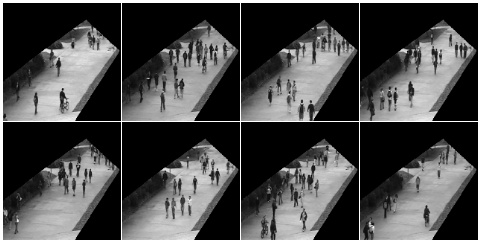
\includegraphics[width=0.8\textwidth]{images/testucsd}}
	\caption{Real UCSD images after being masked and resized.}
	\label{fig:testucsd}
\end{figure}


\indent We will use this dataset to first, validate the performance of our model trained with synthetic data, on a real dataset, and then to do a comparison between the work done in \cite{chan2008privacy} and our approach.



\section{Caffe Deep Learning Platform}

Caffe is a clean and modifiable framework for state-of-the-art deep learning algorithms and a collection of reference models. The framework is a BSD-licensed C++ library with Python and MATLAB bindings for training and deployment of general-purpose convolutional neural networks and other deep models on commodity architectures \cite{jia2014caffe}. It powers on-going research projects and large-scale industrial applications in vision, speech and multimedia by CUDA \footnote{CUDA is a parallel computing platform and application programming interface (API) model created by NVIDIA \cite{cuda}, processing over 40 million images a day on a single K40 or Titan GPU \cite{jia2014caffe}.}  GPU computation.

Caffe is composed of two main components, models' architecture and design, and model optimization. In the rest of this section, we present the main components and parameters of both model implementation and optimization.
\subsection{Model Implementation and Design}
The main components of Caffe architecture are outlined below:
\begin{enumerate}

\item \textbf{Data storage:} Caffe stores and communicates data in 4-dimensional arrays called \textit{blobs}. Blobs provide a unified memory interface, holding batches of data, parameters, or parameter updates. Blobs conceal the computational overhead by synchronizing from the CPU host to the GPU device as needed. Figure~\ref{fig:blob} shows the blobs connected to a convolution layer implemented by Caffe.


\begin{figure}[H]
	\centering
	{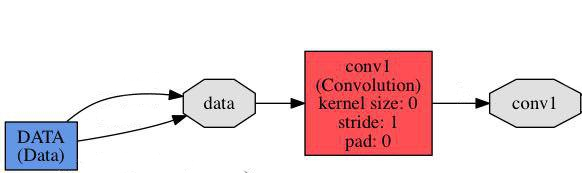
\includegraphics[width=0.7\textwidth]{images/caffeconvlayer}}
	\caption{Input (data) and output (conv1) blobs of a convolution layer in a CNN implemented in Caffe.}
	\label{fig:blob}
\end{figure}


Caffe supports some data sources such as LevelDB or LMDB (Lightning Memory-Mapped Database), HDF5, MemoryData, ImageData, etc. However, large-scale data is stored in LevelDB databases since it reads the data directly from memory \cite{caffe}. 
\item \textbf{Layers:} A caffe layer takes blobs as input and yields one or more as output. In a network (as described in chapter~\ref{subsec:bp}), each layer plays two important roles: a forward pass that takes the inputs and produces the outputs, and a backward pass that takes the gradient with respect to the output, and computes the gradients with respect to the parameters and to the inputs, which are in turn back-propagated to earlier layers \cite{jia2014caffe}.

\indent Caffe supports an exhaustive set of layers, including the followings \cite{jia2014caffe}: 
\begin{enumerate}
	\item Convolution, pooling, fully connected, 
	\item Nonlinearities like rectified
	linear and logistic, local response normalization, element-wise operations, and 
	\item Losses like softmax and hinge
\end{enumerate}
\item \textbf{Networks and run mode:} Caffe ensures the correctness of the forward and backward passes for any directed acyclic graph of layers. A typical network begins with a data layer laying down at the bottom going up to the loss layer that computes tasks' objectives. The network is run on CPU or GPU independent of the model definition. 
\item \textbf{Training a network:} Training phase in Caffe is done by classical stochastic gradient descent algorithm. When training, images and labels pass through different layers lead into the final prediction into a classification layer that produces the loss and gradients which train the whole network. Figure~\ref{fig:caffe} illustrates a typical example of a Caffe network. 


\indent Finetuning, the adaptation of an existing model to new architectures or data, is a standard method in Caffe. Caffe  finetunes the old model weights for the new task and initializes new weights as needed. This capability is essential for tasks such as knowledge transfer \cite{donahue2013decaf}, object detection \cite{girshick2014rich}, and object retrieval \cite{guadarrama2014open}, \cite{jia2014caffe}.  
\end{enumerate}


\begin{figure}[H]
	\centering
	{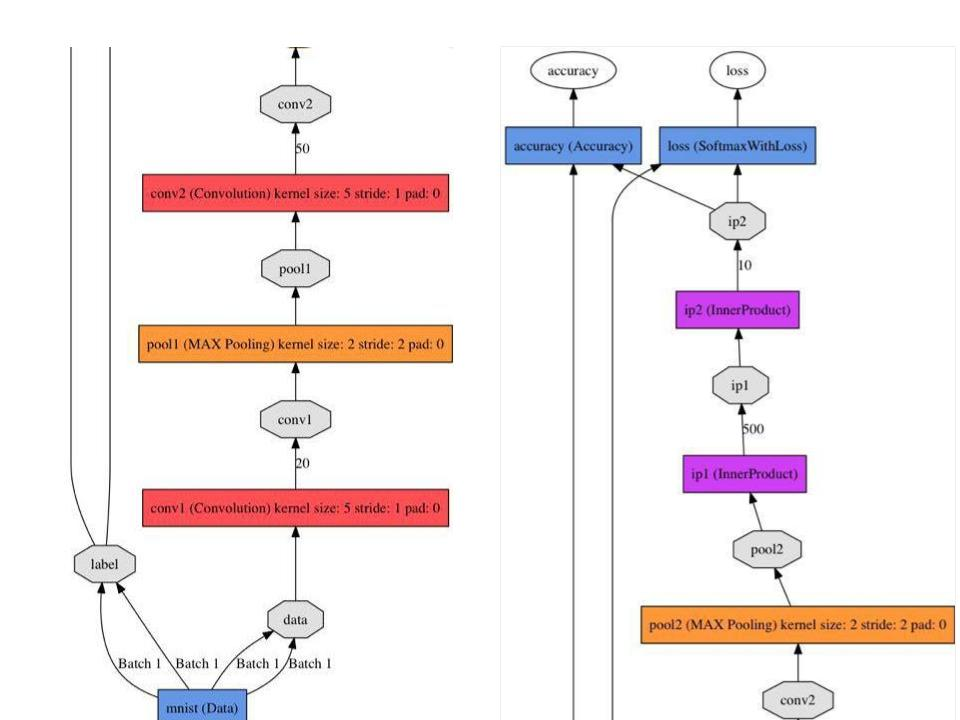
\includegraphics[width=0.9\textwidth]{images/le2col}}
	\caption{From bottom-left to top-right, Lenet architecture for MNIST digit classification example of a Caffe network, where boxes represent layers and octagons represent data blobs produced by or fed into the layers \cite{jia2014caffe}.}
	\label{fig:caffe}
\end{figure}

\textbf{Justification}: We decided to use Caffe because, it addresses computation efficiency problems (as likely the fastest available implementation of deep learning frameworks at the time of performing this study, adheres to software engineering best practices, providing unit tests for correctness and experimental rigor and speed for deployment. It is also well-suited for research use, due to the well-implemented modularity of the code, and the clean separation of network definition (usually the novel part of deep learning research) from actual implementation\cite{jia2014caffe}. In addition, it provides a python wrapper which exposes the solver module for easy prototyping of new training procedures. 

\subsection{Model Optimization}

Our work in general is an optimization problem since we project the results as loss functions we try to minimize. For this reason, model optimization methods have a critical impact on the performance of the model. In Caffe, \textit{Solver} file orchestrates optimization by coordinating the network's forward inference and backward gradients to form parameter updates that attempt to improve the loss. Among Caffe solver methods, we use stochastic gradient descent (explained in chapter~\ref{subsec:sgd}). The use of SGD in deep convolutional neural network setting is motivated by the high cost of running back propagation over the full training set. SGD can overcome this cost and still lead to fast convergence. 

Although Caffe provides several optimization methods, in this section we briefly describe merely optimization methods and \textit{hyper-parameters}\footnote{Hyper-parameters govern the underlying system on a "higher level" than the primary parameters of interest. They are not model parameters that are learned during training phase and instead, they are set by the designer a priori.} incorporated in our proposed algorithms.


\subsubsection{Batch Size}

Since Caffe is trained using stochastic gradient descent, at each iteration, it computes the (stochastic) gradient of the parameters with respect to the training data and updates the parameters in the direction of the gradient. On the other hand, to compute the gradient w.r.t the input data, we need to evaluate all training samples at each iteration which is prohibitively time-consuming, specially when we are dealing with a great amount of data. 

\indent In order to overcome this issue, SGD approximates the exact gradient, in a stochastic manner, by sampling only a small portion of the training data at each iteration. This small portion is the \textit{batch}. In other words, the batch size defines the amount of training data we feed to the network at each iteration. The larger the batch size, the more accurate the gradient estimate at each iteration will be. 

\subsubsection{Learning Rate}
\label{learning rate}
Learning rate is a decreasing function of time. It's a common practice to decrease the base learning rate (base\_lr) as the optimization/learning process progresses. In Caffe, different learning policies exist among which we tried the followings:
\begin{itemize}
\item \textit{\textbf{Fixed}:} which always returns the base learning rate.

\item \textit{\textbf{inv}:} which returns $$base\_lr \times (1 + \gamma \times iteration) ^ {(-Power)}$$ where:\\\textit{ $\gamma$: the factor learning rate drops by.}\\\textit{power: another factor that learning rate drops by.}

\item \textit{\textbf{step}:} that returns $$base\_lr \times \gamma ^ {floor(\frac{iteration}{step})}$$ where:\\ \textit{$\gamma$: the factor learning rate drops by.}\\\textit{step: the number of iteration at which the learning rate drops.} 
\item \textit{\textbf{multi-step}:} similar to step but it allows non uniform steps defined by step value.
\end{itemize}
Although there are numerous empirical studies and rules of thumb to treat learning rate \cite{senior2013empirical,yu1995dynamic,minai1990acceleration}, basic learning rate and learning policy are highly problem-dependent.  

\subsubsection{Weight Decay}


As a part of Back Propagation and a subset of regularization methods, \textit{weight decay} adds a penalty term to the error function by multiplying weights to a factor slightly less than 1 after each update. 

 It has been observed in numerical simulations that a weight decay can improve generalization in a feed-forward neural network. It is proven that weight decay has two effects in a linear network. Firstly, it suppresses any irrelevant components of the weight vector by choosing the smallest vector that solves the learning problem. Secondly, if the size is chosen correctly, a weight decay can suppress some of the effects of static noise on the targets, which improves generalization significantly \cite{moody1995simple}. 

\subsubsection{Momentum}
%\todo{doesn't it belong to state-of-the art / implementation??cant put it in implementation cuz its built-in caffe and I just set the value. Hence, I thought they are better off here since they belong also to model optimization?}
One of the potential problems with stochastic gradient descent is having oscillations in the gradient, since not all examples are used for each calculation of the derivatives. This can cause slow convergence of the network. One strategy to mitigate this problem is the use of \textit{Momentum}. The momentum method introduced by \citeauthor{polyak1964some}, \citeyear{polyak1964some}, is a first-order optimization method for accelerating gradient descent that accumulates a velocity vector in directions of persistent reduction in the objective across iterations. Given an objective function $f(\theta)$ to be minimized, momentum is given by:
\begin{equation}
	\label{eq:t}
	\begin{aligned}
		\nu_{t+1} = \mu\nu_t - \alpha\nabla 
	\end{aligned}
\end{equation}
\begin{equation}
	\label{eq:t}
	\begin{gathered}
	\theta_{t+1} = \theta_t + \nu_{t + 1}
	\end{gathered}
\end{equation}
where $\alpha > 0$ is the learning rate, $\mu \in [0,1]$ is the momentum coefficient, and $\nabla f(\theta_t)$ is the gradient at $\theta_t$ \cite{sutskever2013importance}. 

For example, if the objective has a form of a long shallow ravine leading to the optimum and steep walls on the sides, standard SGD will tend to oscillate across the narrow ravine since the negative gradient will point down one of the steep sides rather than along the ravine towards the optimum \cite{sgd}. The objectives of deep architectures have this form near local optima and thus standard SGD can lead to very slow convergence particularly after the initial steep gains. 

Momentum, by taking the running average of the derivatives, by incorporating the previous update in the update for the current iteration, is one method for pushing the objective more quickly along the shallow ravine \cite{sgd}. 

\subsubsection{Number of Iterations}

In learning process, common convergence criteria are: a maximum number of iteration; a desired value for the cost function is reached; or training until the cost function shows no improvement in a number of iterations. In our implementation, we use the maximum number of iteration as our systems' convergence policy. 
 
The number of iterations plays an important role in the training process. iteration number is in an inverse correlation with the number of instances and also the batch size. In any network, batch size and iteration number compensate for one another. For instance, in case of lack of memory, one option would be to decrease the batch size and increase the number of iterations accordingly.


\section{The Architecture}
\label{imparch}

Having Caffe platform introduced, we propose two CNN-based deep architectures for the analysis we did regarding two learning to count problems, counting the number of even-digits and the number of pedestrians in an image.  
In learning object features for vision tasks and by the use of DCNN, the depth of network plays a crucial role. The deeper the model, the better it learns. However, issues like overfitting\footnote{Overfitting occurs when a statistical model describes random error or noise instead of the underlying relationship, and vice versa for underfitting. } and underfitting should not be left neglected.   
Therefore, in this section, networks' settings and architectures for even-digits and crowd counting problems will be described separately. 

\subsection{Even-digit Counting}
\label{subsubsec:digitarch}

For learning to count even digits problem, since we used MNIST dataset to generate our images, we considered the architecture proposed by \citeauthor{lecun1995comparison} for classic MNIST hand-written digit recognition problem \cite{lecun1995comparison} (shown in figure~\ref{fig:caffe}), as the base of our design. In addition, we took into account the architecture used in state-of-the-art \cite{segui2015learning}. Figure~\ref{santil2cfull} demonstrates this architecture. From there, we modified the architecture to optimize the performance of the network. 
 
\begin{figure}[H]
  \centering
   {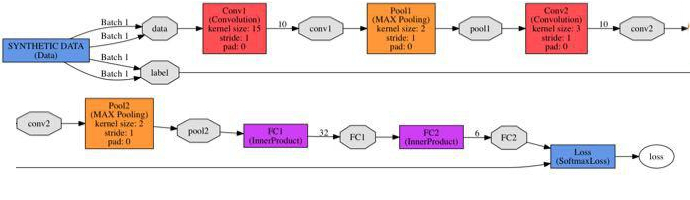
\includegraphics[width=1.\textwidth]{images/santil2cfull}}
  %\end{center}
	\caption{From top-left to bottom-right, the network proposed in \cite{segui2015learning} for Even digits recognition task.}
	\label{santil2cfull}
\end{figure}

\noindent In a similar experiment with maximum 5 digits in images, \citeauthor{segui2015learning} in \cite{segui2015learning} defined a four layers CNN with two convolutional layers for classifying even digits present in images. Each convolutional layer consists of several elements: a set of convolutional filters, ReLU non-linearities, max pooling layers and normalization layers. The first convolutional layer outputs 10 filters of dimensions $15\times15$, and the second convolution layer has 10 filters, each of size $3\times3$. Each convolution layer is followed by a max-pooling layer with a $2\times2$ kernel. The output of last pooling layer is fed to two fully-connected layers with respectively 32 and 6 number of outputs. They also used Softmax loss layer on top of their architecture to compute the multinomial logistic loss layer\footnote{This function displays a similar convergence rate to the hinge loss function, and since it is continuous, gradient descent methods can be utilized. Also, functions which correctly classify points with high confidence are penalized less. This structure is highly sensitive to outliers in the data.}. Table~\ref{santil2c} presents the main components of the network designed by \cite{segui2015learning}. 

\begin{table}[H]
	\centering
	\begin{tabular}{ |p{2cm}|p{2cm}| }
	\hline 
	\multicolumn{2}{|c|}{\textbf{Network parameters}} \\
	\hline
	\hline
	\textbf{Layers} & \textbf{setting }\\
	\hline
	Conv1 & $10\times15\times15$\\
	\hline
	Pool1    & $max(2\times2)$ \\
	\hline
	Conv2 & $10\times3\times3$\\
	\hline
	Pool2 &    $max(2\times2)$ \\
	\hline
	FC1 & 32 outputs \\
	\hline
	FC2 & 6 outputs \\
	\hline
	\end{tabular}
		\caption{The DCNN proposed by \cite{segui2015learning} for learning the number of even digits present in the images.}
		\label{santil2c}
\end{table}
 

\noindent However, in our implementation, due to higher complexity, we decided to apply a deeper CNN with more parameters. In our network, the data layer fetches the images and labels from the disk, passes it through the first convolutional layer with 20 filters, each of size $15\times15$ followed by a ReLU non-linearity and LRN normalization layer. Then the output is max-pooled by the  kernel size of $2\times2$. This process repeats again for the second convolutional layer with having 50 filters of size $5\times5$ and the last convolutional layer with 50 filters with kernel size $3\times3$. No pooling layer follows the last convolution layer. In all convolution and pooling layers, the \textit{stride} = 1 and \textit{padding}\footnote{Zero padding is a simple concept; it simply refers to adding zeros to end of an image to increase its length.} = 1 are considered (see section~\ref{convlayer} for more explanation regarding padding and stride). 

\noindent the output of the second pooling layer is fed to three fully connected (inner product) layers with respectively 128, 64 and 1 number of outputs (since the problem is approached as a regression task). Also the first and second fully connected layers are followed by ReLU non-linearity. 


However, a well-designed network cannot solely guarantee an optimal performance for the model. The responsibilities of learning are divided between the network for yielding loss and gradients, and the optimization methods (solver) and parameters for overseeing the optimization and generating parameter updates. Among Caffe solvers, as described in section~\ref{subsec:sgd}, we use Stochastic Gradient Descent optimization method. Apart from solver method, the solver parameters (network's hyper-parameters) need to be set attentively in order to optimize the model performance. Therefore, to optimize the model performance, the networks' hyper-parameters are set as below while table~\ref{hypers} provides a summary of the hyper-parameters' settings. 
\begin{itemize}

\item \textbf{Batch size:} Due to the non-complex and low-resolution dataset we are training on, we were able to use batches of size 256 for our training and testing phases.

\item \textbf{Learning rate:} After trying different initial values in range of $(10^{-6}, 1)$, we set the basic learning rate to $\alpha = 0.0001$. However, for our experiment we chose \textit{multi-step} learning policy in which, after each \textit{stepsize}=40000 iterations, the learning rate drops by the rate of Gamma $\gamma = 0.1$. This initialization is based on rules of thumb used in \cite{krizhevsky2012imagenet}.

\item \textbf{Momentum:} We use momentum $\mu = 0.9$. Because, momentum setting $\mu$ effectively multiplies the size of our updates by a factor of $\frac{1}{1-\mu}$. Hence, changes in momentum and learning rate ought to be accompanied with an inverse correlation. When momentum $\mu = 0.9$, we have an effective update size of 10 since we also drop the learning rate by the factor of $\gamma= 0.1$.

%
%\item \textbf{Momentum:} We use momentum $\mu = 0.9$. This selection also is based on trial and error. As momentum value $\mu$ effectively multiplies the size of our updates by a factor of $\frac{1}{1-\mu}$. Hence, changes in momentum and learning rate ought to be accompanied with an inverse correlation. When momentum $\mu = 0.9$, we have an effective update size of 10 since we also drop the learning rate by the factor of Gamma $\gamma= 0.1$.

\item \textbf{Weight decay:} Weight decay as a penalty term to the error function, has a constant value of 0.0005. This decay constant is multiplied to the sum of squared weights.

\item \textbf{Iterations:} Given the time and hardware we had, we managed to let the system train for 1,600,000 iterations.

\end{itemize}

\begin{table}[H]
	\centering
	\begin{tabular}{ |p{3.8cm}|p{1.7cm}| }
	\hline 
	\multicolumn{2}{|c|}{\textbf{Network hyper-parameters}} \\
	\hline
	\hline
	\textbf{Hyper-parameters} & \textbf{setting }\\
	\hline
	Learning rate & 0.0001\\
	\hline
	Learning policy    & \textit{Multi\_step} \\
	\hline
	Momentum & $\mu = 0.9$\\
	\hline
	Weight decay & 0.0005 \\
	\hline
	Batch size & 256 \\
	\hline
	Iterations & 1600000 \\
	\hline
	\end{tabular}
		\caption{Proposed settings for network's hyper-parameters for counting number of even digits task.}
		\label{hypers}
\end{table}
 

\noindent We should also mention that at the top layer of the network, we used Euclidean Loss layer to compute the euclidean distance between the predictions and the ground truth.  Figure~\ref{fig:l2cNet} shows a scheme of the architecture while table~\ref{ourltc} summarizes the design. 
		\begin{table}[H]
			\centering
			\begin{tabular}{ |p{2cm}|p{2cm}| }
			\hline 
			\multicolumn{2}{|c|}{\textbf{Network parameters}} \\
			\hline
			\hline
			\textbf{Layers} & \textbf{setting }\\
			\hline
			Conv1 & $20\times15\times15$\\
			\hline
			Pool1    & $max(2\times2)$ \\
			\hline
			Conv2 & $50\times5\times5$\\
			\hline
			Pool2    & $max(2\times2)$ \\
			\hline
			Conv3 & $50\times3\times3$\\
			\hline
			IP1 & 128 outputs \\
			\hline
			IP1 & 64 outputs \\
			\hline
			IP2 & 1 outputs \\
			\hline
			\end{tabular}
				\caption{Proposed architecture's settings.}
				\label{ourltc}
		\end{table}
		 
%    \end{minipage} 
%        %\caption{Global caption}
%\end{table}



\begin{figure}[H]
  \centering
   {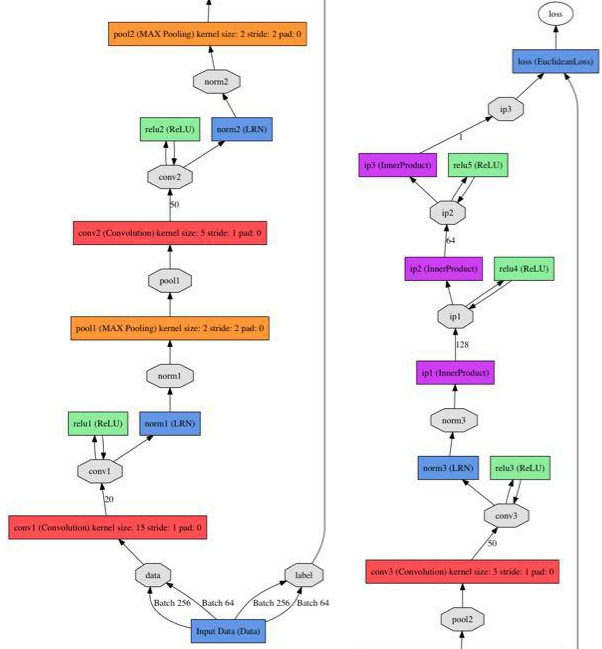
\includegraphics[width=0.9\textwidth]{images/ohoh}}
  %\end{center}
	\caption{From bottom-left to top-right, the proposed network architecture for Even digits counting task}
	\label{fig:l2cNet}
\end{figure}

%\todo{this is a useless statement, unless you go into detail what heuristics you've used. justification needed for your choise. so beef it up here between these two sentences}
The architecture has been designed intuitively and based on a heuristic approach where we tried different values for each hyper-parameter at a time and selected the values that provided us with an improvement in the performance of the network. Hence, one may be able to improve the performance by implementing a different architecture or with another settings for the hyper-parameters of the network. 

\subsection{Crowd Counting}
\label{subsec:ucsdarch}

For the task of counting pedestrians, due to the more complex images than the previous task, we designed a deeper architecture. Moreover, we applied the same settings of hyper-parameters to a different architecture. However, as a reminder, table~\ref{hypar2} summarizes the network's settings for the hyper-parameters.

\begin{table}[H]
	\centering
	\begin{tabular}{ |p{3.8cm}|p{1.7cm}| }
	\hline 
	\multicolumn{2}{|c|}{\textbf{Network hyper-parameters}} \\
	\hline
	\hline
	\textbf{Hyper-parameters} & \textbf{setting }\\
	\hline
	Learning rate & 0.0001\\
	\hline
	Learning policy    & \textit{Multi\_step} \\
	\hline
	Momentum & $\mu = 0.9$\\
	\hline
	Weight decay & 0.0005 \\
	\hline
	Batch size & 256 \\
	\hline
	Iterations & 1600000 \\
	\hline
	\end{tabular}
		\caption{Proposed settings for network's hyper-parameters for counting pedestrians.}
		\label{hypar2}
\end{table} 

As a baseline, we considered state-of-the-art architecture designed by \citet{segui2015learning} for counting the number of pedestrians in the images. As shown in figure~\ref{santiucsdnet}, in their work, they used a five layer architecture CNN with two convolutional layers followed by three fully connected layers. Convolutional layers contain their main elements (ReLU and LRN layers), and each outputs 8 filters with kernel sizes $9\times9$ and $5\times5$ respectively. 

\begin{figure}[H]
  \centering
   {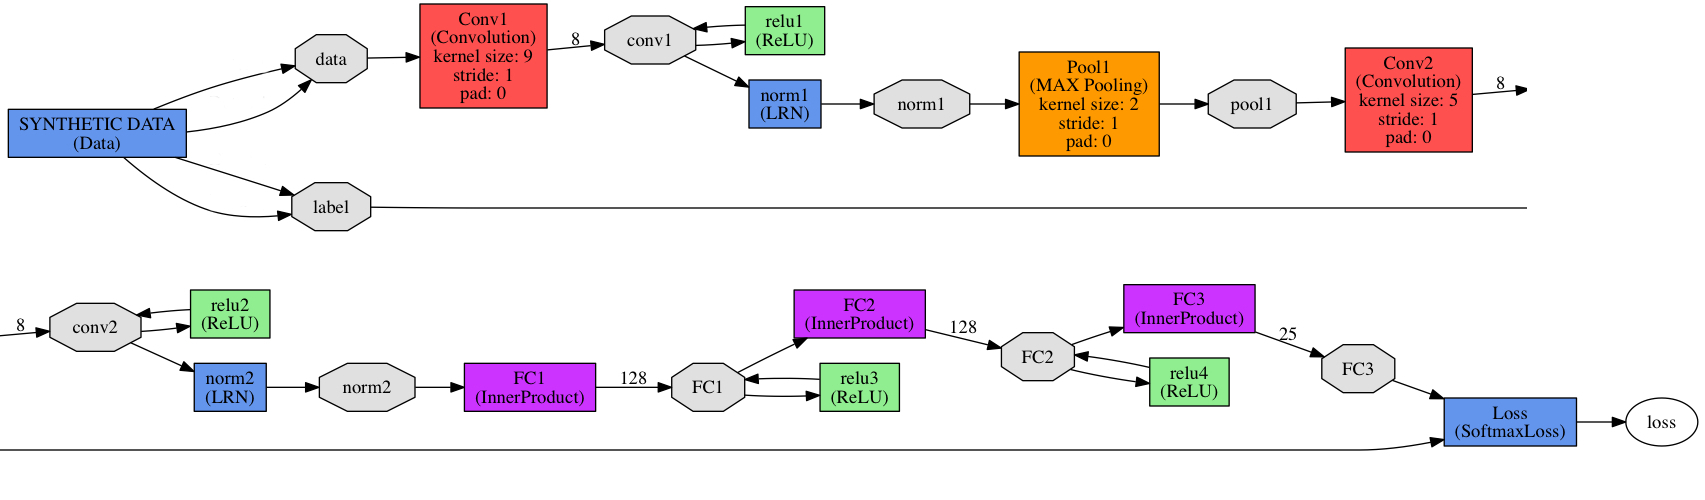
\includegraphics[width=1.00\textwidth]{images/santiucsd}}
  %\end{center}
	\caption{From top-left to bottom-right, the DCNN proposed by \cite{segui2015learning} for learning to count the number of pedestrians in a walkway.}
	\label{santiucsdnet}
\end{figure}

They applied only one max-pooling layer and after the first convolutional layer in their design. Finally, three fully connected layers with number of outputs 128, 128 and 25 classify the output of the network into 25 classes (maximum pedestrians in the images) of the number of people in the image. Similar to the previous task, a softmax loss layer projects the performance of the model.   
Table~\ref{santiarch} describes a summary of their network.

\begin{table}[H]
	\centering
	\begin{tabular}{ |p{2cm}|p{2cm}| }
	\hline 
	\multicolumn{2}{|c|}{\textbf{Network parameters}} \\
	\hline
	\hline
	\textbf{Layers} & \textbf{setting }\\
	\hline
	Conv1 & $8\times9\times9$\\
	\hline
	Pool1    & $max(2\times2)$ \\
	\hline
	Conv2 & $8\times5\times5$\\
	\hline
	FC1 & 128 outputs \\
	\hline
	FC2 & 128 outputs \\
	\hline
	FC3 & 25 outputs \\
	\hline
	\end{tabular}
		\caption{The deep CNN proposed by \citealt{segui2015learning} for learning the number of pedestrians in a walkway.}
		\label{santiarch}
\end{table}


\noindent However, since up to 29 pedestrians are present in our images with high amount of overlapping, in our design we added one convolutional layer to the base architecture. We also increased the number of parameters in the network. In our architecture, the data blobs pass through 4 convolutional layers. The first convolutional layer has 10 filters, each with $15\times15$ kernel. The second convolution layer contains 10 filters of dimensions $11\times11$. Respectively for the third and fourth convolution layers, kernels of sizes $9\times9$ and $5\times5$  provide 0 filters for each layer. Similar to the previous model, each convolutional layer is followed by ReLU non-linearity layer and LRN normalization layer. Also the stride and padding values for all the convolutional layers are respectively equal to 1 and 0. Table~\ref{ourpednet} shows the main structure of this architecture. 

\begin{table}[H]
	\centering
	\begin{tabular}{ |p{2cm}|p{2cm}| }
	\hline 
	\multicolumn{2}{|c|}{\textbf{Network parameters}} \\
	\hline
	\hline
	\textbf{Layers} & \textbf{setting }\\
	\hline
	Conv1 & $10\times15\times15$\\
	\hline
	Pool1 & $max(2\times2)$ \\
	\hline
	Conv2 & $10\times11\times11$\\
	\hline
	Pool2 & $max(2\times2)$ \\
	\hline
	Conv3 & $20\times9\times9$\\
	\hline
	Conv4 & $20\times5\times5$\\
	\hline
	IP1   & 128 outputs \\
	\hline
	IP2   & 64 outputs \\
	\hline
	IP3   & 1 outputs \\
	\hline
	\end{tabular}
		\caption{Proposed architecture's settings.}
		\label{ourpednet}
\end{table}
%\todo{ok, i really want a figure showing the architecture of the network you've designed. it should show the layers, kernels, ... a zoom-in, no full-scale representation needed, just a cutout}

\indent In order to not lose information, we used merely two pooling layers for the first two convolutional layers. Each pooling layer has a kernel size of $2\times2$ with $stride = 1$  and $padding = 0$. Figure~\ref{fig:ucsdnet} illustrates the proposed architecture. 

\begin{figure}[H]
  \centering
   {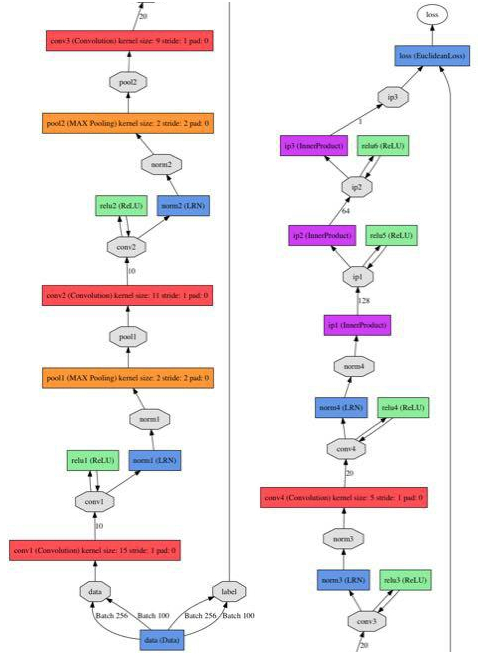
\includegraphics[width=0.65\textwidth]{images/uscdmine}}
  %\end{center}
	\caption{Proposed network architecture for learning the number of pedestrians in the image.}
	\label{fig:ucsdnet}
\end{figure}

As you may see in figure~\ref{fig:ucsdnet} above, there are three fully connected layers to regress the number of pedestrians in images. The first fully connected layers has 128 output units, and the second layer outputs 64 units. The last layer however, with solely one output, passes the models' prediction of the number of pedestrians to the Euclidean loss layer to calculate the sum of squares of differences of its two inputs, the true labels and predictions. 
%In figure~\ref{fig:ucsdnet}, an illustration of this architecture has been presented.

To the best of our knowledge, the designed architectures outperform other architectures we tried previously (a different range of architectures starting from 1 up to 5 convolutional layers with different settings), while also fastening the training phase . However, apart from the basic knowledge about network architectures, hyper-parameters initialization and some rules of thumb of successful experiences in similar works, the rest of design has been done intuitively. Therefore, similar to the first architecture (problem of counting even digits), there would be other ways to improve the architecture and performance of the model.


